\documentclass[12pt]{article}

\usepackage{hyperref}
\usepackage{titlesec}
\usepackage{amsthm,amssymb}
\usepackage{amsmath}
\usepackage{graphicx}
\usepackage{minted}
\usepackage{caption} % Required for specifying captions to tables and figures
\usepackage{comment}
\usepackage[section]{placeins}


\graphicspath{ {images/} }

\title{CS3210 Assignment 2 Report}
\date{\today}
\author{Mok Wei Xiong, Edmund (A0093960X)}

\begin{document}
% title
\maketitle

\section{Outline}

One simple way to find a nonce that gives a valid digest is simply to try all possible nonces, and return as soon as we determine that a nonce does indeed lead to a valid digest. Since it is difficult to determine if a nonce will actually give a valid digest or not, I just treat the hashing function as a black box and try all possible nonces starting from 0, incrementing the nonce to try on each \textit{unsuccessful} digest.

\bigbreak \noindent It is easy to parallelize this strategy across multiple threads on a GPU. Each thread can be assigned an initial nonce from $0$ to \verb!num_threads!$- 1$, and each thread will then check if their respective nonces can give valid digests. On each \textit{unsuccessful} nonce that does not give a valid digest, each thread will increment its own nonce by \verb!num_threads!, and this will allow every thread to try a unique set of nonces, ensuring that there is no wasted or duplicate work where multiple threads check the same nonce. Eventually, when a thread has found a valid nonce, it will \textit{signal} to the other threads to stop searching further, and the desired output will be shown on the screen.

\bigbreak \noindent I chose to implement this strategy since it is simple to implement and is also in line with the data parallelism model that CUDA follows, as opposed to a task parallelism model. 

\section{Implementation Specifics}

I will describe some of the specifics in my implementation, following the strategy as mentioned in the previous section.

\subsection{Initialisation Phase}

In order for each CUDA thread to check a nonce, it requires the timestamp, previous digest, and NUSNET ID. The timestamp is captured in the host and the same timestamp is used throughout the entire nonce finding procedure so that we can eventually find a nonce that is valid. Otherwise, if the timestamp keeps changing it is possible that my strategy may not find a valid nonce.

\bigbreak \noindent The host first assembles the timestamp, previous digest and NUSNET ID into an array \verb!input!, and copies this data into another array in the device global memory \verb!d_input! for the CUDA threads to access. The target value is also copied over into device global memory \verb!d_target! in the same way. Finally, some device global variables are initialised to keep track of the state, such as \verb!d_found! to keep track of whether a nonce has been found, \verb!d_nonce! and \verb!d_hash! to hold the final nonce and digest of a valid nonce, so that it can be copied over to host memory at the end.

\bigbreak \noindent The host then runs the kernel \verb!find_nonce_kernel! that will begin the actual nonce finding procedure.

\subsection{Preparation Phase}

Before each thread can actually begin, it determines its initial nonce to check by using finding its own \verb!thread_id!, and also calculating the total \verb!num_threads!.

\bigbreak \noindent Furthermore, each thread will copy the \verb!d_input! array from global memory to its own thread local memory for faster memory access. The same is done for copying the global \verb!d_target! to local memory. Finally, each thread will fill their own local input array with its initial nonce.

\subsection{Exploration Phase}

Each thread will then loop while \verb!d_found!, the flag signalling whether any thread has found a valid nonce, is 0, and check its own nonce. If it is invalid, increment its nonce by \verb!num_threads! and check again. If it is valid, then this thread will do an \verb!atomicAdd! to \verb!d_found!. This ensures that if it happens that multiple threads found a nonce at the same time, only one (the one whose \verb!atomicAdd! returns 0) will update the \verb!d_nonce! and \verb!d_hash! global memory variables and there will not be any race conditions or data corruption.

\bigbreak \noindent At this point, all other threads while looping will see that \verb!d_found! is already set, and break from their loops.

\subsection{Ending Phase}

Back on the host, we know that at this point there must be a valid nonce already. Thus, the nonce \verb!d_nonce! and digest \verb!d_hash! is copied from device global memory to host memory. Finally, the NUSNET ID, timestamp, nonce and digest are printed out as required.

\section{Measurements}

In the following measurements, I used a fixed timestamp of \textbf{1538352000} to ensure that the measurements are consistent in trying to find a valid digest of similar difficulty throughout. I have also fixed the previous digest as \textbf{3210327c68bb9409c4aa5806a4c018e26dcd2ca599a5cbccfaf09c886f701b71}
 and target value to be \textbf{1474976710656}. The target value was set to be smaller than the sample target value provided since the sample target value was not that difficult and did not yield any meaningful measurements on the Jetson TX2 board, finishing in $ < 200$ ms each time.
 
 
\subsection{Investigating varying number of threads}

These measurements were made on the Jetson TX2.

\begin{table}[]
\begin{center}
\begin{tabular}{|l|l|l|l|l|l|l|l|l|l|}
\hline
Grid Size & 1 & 1 & 1 & 1 & 1 & 2 & 4 & 10 & 20 \\ \hline
Block Size & 1 & 32 & 64 & 128 & 256 & 256 & 256 & 256 & 256 \\ \hline
Measurements & 55.993 & 2.308 & 1.494 & 1.37 & 0.629 & 0.438 & 0.348 & 0.224 & 0.242 \\ \hline
 & 55.597 & 2.091 & 1.165 & 1.124 & 0.468 & 0.43 & 0.574 & 0.249 & 0.247 \\ \hline
 & 55.908 & 1.982 & 1.508 & 0.678 & 0.481 & 0.417 & 0.34 & 0.363 & 0.231 \\ \hline
Minimum & \textbf{55.597} & \textbf{1.982} & \textbf{1.165} & \textbf{0.678} & \textbf{0.468} & \textbf{0.417} & \textbf{0.34} & \textbf{0.224} & \textbf{0.231} \\ \hline
\end{tabular}
\end{center}
\caption{Measurements from 1 to 5120 threads (Jetson TX2)}

\begin{center}
\begin{tabular}{|l|l|l|l|}
\hline
Grid Size & 30 & 35 & 40 \\ \hline
Block Size & 256 & 256 & 256 \\ \hline
Measurements & 0.202 & 0.887 & 1.191 \\ \hline
 & 0.219 & 0.572 & 1.258 \\ \hline
 & 0.218 & 0.489 & 0.963 \\ \hline
Minimum & \textbf{0.202} & \textbf{0.489} & \textbf{0.963} \\ \hline
\end{tabular}
\end{center}
\caption{Measurements from 7680 to 10240 threads (Jetson TX2)}
\end{table}

\begin{center}
	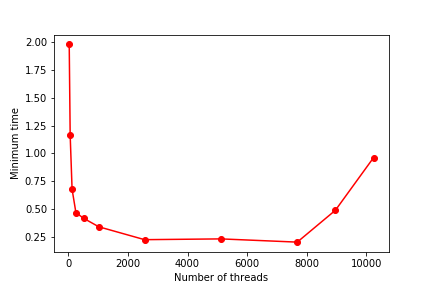
\includegraphics[scale=0.8]{images/threads_vs_time}
	\captionof{figure}{Plot of number of threads vs time (exclude 1 thread)}
\end{center}

\bigbreak \noindent From the measurements above, it is clear that the parallelism is very effective in speeding up the nonce finding procedure, yielding a speedup of $55.597/1.982 = 28.1$ when using 32 threads and even $55.597/0.202 = 275.2$ when using a configuration of $30 * 256$.

\bigbreak \noindent There is also a general trend of increasing performance as the number of threads increases from 0 to 8000 threads as can be seen in Figure 1. This can be explained by the increasing parallelism possible as the number of threads is increased, where we can fully exploit every core and SM in the device to  maximize the parallelism.

\bigbreak \noindent After a certain point (8000 threads), increasing the number of threads seems to hurt rather than help the performance of the parallel program. This is similar to too many threads may hurt performance when programming on a CPU, and thus could perhaps be due to reasons like too much overhead in context switching between threads compared to the amount of work done by the increased number of threads.

\subsubsection{Maximum number of threads in block}

\bigbreak \noindent Another interesting thing is that as I was trying to increase the number of threads in the block, the maximum I could go was 256. As such, I had to keep the number of threads per block to 256 and increase the number of blocks in order to increase the number of threads. There was actually no error messages and I was able to compile it successfully using \verb!make! and even run the executable. The only reason I spotted something wrong was that the code returned a rubbish value for the nonce and digest.

\bigbreak \noindent I think one possible reason could be due to memory usage, since for my implementation each thread will use a lot of local memory to store the input for hashing, the target value, etc., which adds up to at least 1KB per thread. However, it is also weird that I am allowed to simply increase the number of blocks instead of the number of threads per block but this issue does not occur. I'm not exactly clear what is the cause of this problem, and seems like it requires more in-depth analysis of CUDA architecture and limits.

\subsection{Investigating different block and grid sizes}

I also investigated different configurations of block and grid sizes for the same total number of threads to see if performance is affected. The measurements were made for fixed total of 64, 128 and 256 threads. These are once again measured from the Jetson TX2.

\begin{table}[]
\begin{center}
\begin{tabular}{|l|l|l|}
\hline
Grid Size & 1 & 2 \\ \hline
Block Size & 64 & 32 \\ \hline
Measurements & 1.494 & 1.155 \\ \hline
 & 1.165 & 1.172 \\ \hline
 & 1.508 & 1.387 \\ \hline
Minimum & \textbf{1.165} & \textbf{1.155} \\ \hline
\end{tabular}
\end{center}
\caption{Different configurations for 64 threads (Jetson TX2)}

\begin{center}
\begin{tabular}{|l|l|l|l|}
\hline
Grid Size & 1 & 2 & 4 \\ \hline
Block Size & 128 & 64 & 32 \\ \hline
Measurements & 1.37 & 0.697 & 1.059 \\ \hline
 & 1.124 & 1.269 & 0.729 \\ \hline
 & 0.678 & 0.847 & 0.855 \\ \hline
Minimum & \textbf{0.678} & \textbf{0.697} & \textbf{0.729} \\ \hline
\end{tabular}
\end{center}
\caption{Different configurations for 128 threads (Jetson TX2)}

\begin{center}
\begin{tabular}{|l|l|l|l|l|}
\hline
Grid Size & 1 & 2 & 4 & 8 \\ \hline
Block Size & 256 & 128 & 64 & 32 \\ \hline
Measurements & 0.629 & 0.54 & 0.501 & 0.562 \\ \hline
 & 0.468 & 0.673 & 0.44 & 0.587 \\ \hline
 & 0.481 & 0.42 & 0.404 & 0.429 \\ \hline
Minimum & \textbf{0.468} & \textbf{0.42} & \textbf{0.404} & \textbf{0.429} \\ \hline
\end{tabular}
\end{center}
\caption{Different configurations for 256 threads (Jetson TX2)}
\end{table}

\bigbreak \noindent From Tables 3 to 5, it does not seem like the different configurations within a fixed total number of threads has much impact on the performance, other than small variations that are likely not significant.

\bigbreak \noindent This is not really surprising since the total number of threads running concurrently is still the same, so the grid and block configurations really only affect the ease of data access. In this application, that does not really come into play since I don't really use the grid and block index to access the data for a specific thread, so the configuration is not really essential here.

\bigbreak \noindent Regrettably, I did not measure configurations where the block size is smaller than the warp size of 32, as I had initially intended to make only fair comparisons where the warp size is fully fulfilled. For example, configurations like grid size 4 * block size 16, or grid size 8 * block size 8. In such cases, we would expect these configurations to be noticeably slower than their other counterparts where the block size is at least $\geq$ warp size of 32. Since in such configurations, the block size is $<$ warp size, the number of threads executing simulateneously is not maximized, so the parallelism will not be maximized and hence the performance will surely be worse.

\subsection{Investigating different hardware}

I attempted to run the same performance measurements on increasing number of threads for the Tesla V100 on the compute cluster \verb!xgpc6!, but got really weird measurements. I expected the Tesla V100 to perform much better than the Jetson TX2 but it actually performed worse on every measurement.

\bigbreak \noindent One possible explanation is due to other users running processes on the compute clusters, which affected my measurements. Running \verb!nvidia-smi! showed that there were no other processes, but when I ran \verb!ps aux! I could actually see other users running other processes. On the other hand, I was able to secure usage of the Jetson TX2 in the lab and checked that there were no other users using while I was doing my measurements.

\begin{table}[]
\begin{center}
\begin{tabular}{|l|l|l|l|l|l|l|l|l|l|}
\hline
Grid Size & 1 & 1 & 1 & 1 & 1 & 2 & 4 & 10 & 20 \\ \hline
Block Size & 1 & 32 & 64 & 128 & 256 & 256 & 256 & 256 & 256 \\ \hline
Measurements & 26.971 & 2.272 & 1.927 & 1.939 & 1.6191 & 1.79 & 5.852 & 2.175 & 3.548 \\ \hline
 & 26.968 & 2.249 & 1.891 & 1.727 & 1.638 & 1.549 & 5.788 & 3.525 & 4.08 \\ \hline
 & 27.219 & 2.288 & 1.313 & 1.735 & 1.631 & 1.788 & 5.755 & 3.557 & 4.073 \\ \hline
Minimum & \textbf{26.968} & \textbf{2.249} & \textbf{1.313} & \textbf{1.727} & \textbf{1.631} & \textbf{1.549} & \textbf{5.755} & \textbf{3.557} & \textbf{3.548} \\ \hline
\end{tabular}
\end{center}
\caption{Measurements from 1 to 5120 threads (Tesla V100)}

\begin{center}
\begin{tabular}{|l|l|l|l|}
\hline
Grid Size & 30 & 35 & 40 \\ \hline
Block Size & 256 & 256 & 256 \\ \hline
Measurements & 4.389 & 5.542 & 4.108 \\ \hline
 & 4.37 & 5.562 & 4.14 \\ \hline
 & 3.262 & 4.687 & 4.032 \\ \hline
Minimum & \textbf{3.262} & \textbf{4.687} & \textbf{4.032} \\ \hline
\end{tabular}
\end{center}
\caption{Measurements from 7680 to 10240 threads (Tesla V100)}
\end{table}

\begin{center}
	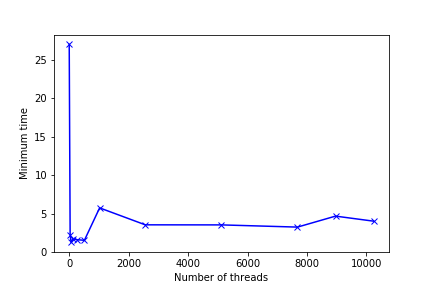
\includegraphics[scale=0.9]{./images/tesla_threads_vs_time}
	\captionof{figure}{Plot of number of threads vs time (Tesla V100)}
\end{center}

\bigbreak \noindent Aside from the higher timings in general for each total number of threads, the general pattern is quite similar to the measurements on the Jetson TX2, with improving performance at the start when increasing the number of threads, and then after a certain point the performance will worsen with more threads.


\subsection{Investigating target difficulty}

I was also curious about how the nonce finding difficulty increases as the target value becomes smaller, so I tried increasing target difficulty and measured the times on both the Jetson TX2 and the Tesla V100.

\begin{table}[]
\begin{center}
\begin{tabular}{|l|l|}
\hline
Target Label & Target Value \\ \hline
A & 281474976710656 \\ \hline
B & 81474976710656 \\ \hline
C & 1474976710656 \\ \hline
D & 474976710656 \\ \hline
E & 74976710656 \\ \hline
F & 4976710656 \\ \hline
\end{tabular}
\end{center}
\caption{Target Label and actual Target Value for Table 7}

\begin{center}
\begin{tabular}{|l|l|l|l|l|l|l|l|}
\hline
 & Target & A & B & C & D & E & F \\ \hline
\begin{tabular}[c]{@{}l@{}}Jetson\\ (30 * 256)\end{tabular} & Nonce & 8166 & 1413225 & 2995741 & 2995741 & 5628618690 & 25080953060 \\ \hline
 & Min Time & \textbf{0.132} & \textbf{0.174} & \textbf{0.202} & \textbf{0.202} & \textbf{18.856} & \textbf{79.755} \\ \hline
\begin{tabular}[c]{@{}l@{}}Tesla\\ (1 * 256)\end{tabular} & Nonce & 8166 & 405318 & 2995741 & 2995741 & 601232501 & 863257849 \\ \hline
 & Min Time & \textbf{0.416} & \textbf{0.478} & \textbf{1.615} & \textbf{1.612} & \textbf{35.055} & \textbf{49.111} \\ \hline
\end{tabular}
\end{center}
\caption{Difficulty vs Time}
\end{table}

\begin{center}
	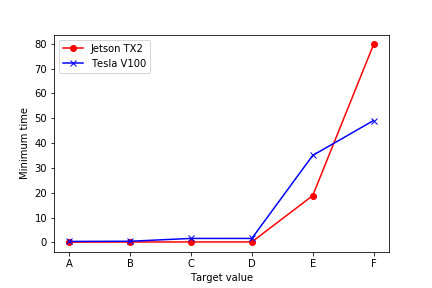
\includegraphics[scale=0.9]{./images/target_difficulty}
	\captionof{figure}{Plot of target value vs time}
\end{center}

\bigbreak \noindent The measurements are performed by using the sample target value as the initial baseline, and then removing a single digit from the target value for each measurement. As we can see from Table 9 and Figure 3, it looks like there is an exponential growth in the time taken to find a valid nonce as the number of digits in the target value decreases.

\bigbreak \noindent I found this quite interesting because even at a target value of 4976710656, which looks like a pretty huge number, the best performance on the Jetson TX2 I have found takes around 80 seconds. Probably the target value equivalent in real world cryptocurrencies will be a lot smaller. If we extrapolate to an even smaller target value (not measured because it would take too long to measure), it demonstrates to me how hard it is to "mine" cryptocurrencies and the reason why miners actually use many GPUs at once to mine in order to increase their chances of successfully mining one.

\bigbreak \noindent From my research, I saw that it is actually possible to use MPI with CUDA so I think a great next step would be to parallize this procedure on multiple GPUs instead of just multiple threads on a single GPU.

\section{Conclusion}

I did not change the SHA256 code and simply used the one that was provided. The hashing function was simply used as a black box to obtain the digest and checked against the target value for the validity of the nonce.

\end{document}
